\chapter{Materiais e Métodos}
\label{chap:materiais_metodos}
O metodologia empregada nos trabalhos de conclusão de curso do Centro Universitário SENAI CIMATEC é executado com base na metodologia TheoPrax que foi desenvolvida pelo instituto Fraunhofer de Tecnologia Química, situado na Alemanha. A sistemática TheoPrax tem como principal objetivo incrementar a motivação da aprendizagem através do desenvolvimento de projetos reais voltados para empresas, proporcionando a integração entre o conhecimento técnico e sua aplicação prática. Para isto, esta estrutura envolve a identificação de uma situação problema ou de uma melhoria no processo ou no produto da empresa, seu estudo e a definição de uma proposta técnica-financeira para implementação da solução.

\section{Metodologia}
\label{sec:metodologia}
A utilização da metodologia Theoprax se restringe apenas ao gerenciamento macro do projeto e não define como a solução proposta deve ser desenvolvida. Sendo assim, o desenvolvimento do projeto, proposto no tópico \ref{sec:objetivo_geral}, será realizado utilizando o procedimento ilustrado na figura \ref{fig:metodologia_diagrama} que foi adaptado da metodologia empregada no BIR (\textit{Brazilian Insitute of Robotics}) para desenvolvimento de projetos de robótica.

\begin{figure}[H]
	\label{fig:metodologia_diagrama}
	\centering
	\caption{Metodologia empregada no desenlvolvimento do projeto solução.}
	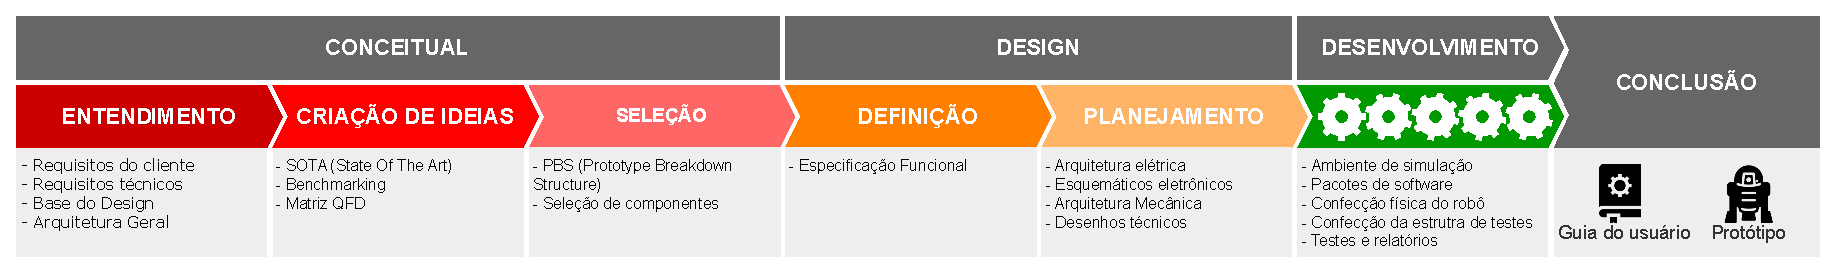
\includegraphics[width=1\textwidth]
	{Figures/metodologia_diagrama}
	\source{Própria Autoria}
\end{figure}	

Conforme figura \ref{fig:metodologia_diagrama}, a metodologia utilizada neste projeto possui 4 etapas: Conceitual, Design, Desenvolvimento e Conclusão. Por conseguinte, cada etapa possui entradas e saídas, que vão se complementando ao longo do desenvolvimento do projeto, as quais serão explicadas nos tópicos seguintes.

\subsection{Conceitual}
\label{subsec:metodologia_conceitual}

A primeira etapa, designada como \textbf{Conceitual}, embora não explicitada no diagrama, possui como entradas as informações provenientes do cliente. Essas informações, tais como o problema proposto e os seus requisitos são utilizadas para o entendimento do projeto, servindo como ponto de partida para formulação da proposta de solução. Diante dessas informações, é possível definir os requisitos técnicos com base nos desejos do cliente (requisitos do cliente); a base do design, que consiste na definição do escopo e o que será necessário para desenvolver o projeto: meios, padrões e os principais componentes (hardware e software); e a arquiterura geral, que fornece uma visão macro de como será a interação entre o hardware e o software do robô. 

Após o entendimento do projeto, passa-se para a criação de ideias. Nesta subetapa, algumas pesquisas são realizadas para ajudar no processo de criatividade e evitar a reimplementação do que já existe no mercado. Assim, utiliza-se o SOTA (\textit{State Of The Art}), documento que aponta as principais pesquisas  e estudos sobre o tema do projeto, referenciando pesquisas acadêmicas já realizadas; e o Benchmarking, que é uma relação oriunda do mercado na qual aponta os competidores para o sistema projetado, incluindo para cada competidor critérios de avaliações importantes para o projeto. Finalizando a subetapa de criação de ideias, tem-se a Matriz QFD (\textit{Quality Functional Deployment}), em que os requisitos do cliente são confrontados com os requisitos técnicos, fornecendo à equipe de desenvolvimento do projeto os principais pontos que deverão receber maior atenção durante a elaboração do projeto. 

Por fim, após o entendimento do projeto e a formulação da ideia, parte-se para a etapa de seleção dos principais componentes do  sistema, em que primeiro elabora-se o PBS (\textit{Prototype Breakdown Structure}), uma representação do projeto com uma visão de subsistemas, apresentado através de um fluxo estruturado.

\subsection{Design}
\label{subsec:metodologia_design}
Com o conceito pré-estabelecido do sistema que será desenvolvido, parte-se para a etapa de \textbf{Design}. Nesta fase, define-se o sistema de maneira mais clara, tendo a especificação funcional como principal elemento. Este documento compreende a explicação  detalhada de cada funcionalidade do robô, contendo a definição, o objetivo, as premissas e as suas entradas e saídas. Devido ao nível de detalhes da especificação funcional, revisões em documentos anteriores, principalmente a arquitetura geral, são realizadas durante esta fase. 

No final da etapa de Design, começa-se o planejamento para o desenvolvimento técnico do projeto. Durante o planejamento é elaborado a arquitetura elétrica do robô (uma visão mais detalhada da arquitetura geral), descrevendo as formas de conexão e os protocolos de comunicação entre os elementos que compõem o sistema; os equemáticos eletrônicos, os quais são utilizados para confecção das PCIs (Placa de Circuito Impresso) que comporão o sistema; a arquitetura mecânica, apresentando os elementos mecânicos do robô; e por fim, os desenhos técnicos mecânicos, utilizados posteriormente para fabricação das peças do protótipo. 

Em conclusão, esta fase é de extrema importância, pois possibilita a geração de documentos que podem ser utilizados para a replicação do projeto. Além do mais, permite mais fluidez no desenvolvimento técnico do robô.

\subsection{Desenvolvimento}
\label{subsec:metodologia_desenvolvimento}

Após a finalização do planejamento, começa-se a etapa de \textbf{Desenvolvimento} do projeto, em que o conceito e as ideias provenientes das etapas anteriores tornam-se concretas. Nesta fase são desenvolvidos e documentados os pacotes de software, os quais englobam tanto a unidade de controle do robô quanto os \textit{drivers} dos sensores, atuadores e elementos de interação com usuário. Muito dos pacotes aqui desenvolvidos, usam a especificação funcional como guia. 

Para auxiliar no processso de desenvolvimento, um ambiente de simulação torna-se elemento vital. O ambiente de simulação permite que ideias sejam propostas e testadas sem a necessidade do uso da plataforma física, acelerando o processo de desenvolvimento num âmbito em que se possui diversas pessoas trabalhando no mesmo sistema. Não menos importante, os simuladores evitam que danos sejam causados ao robô em caso de má implementação de algum algoritmo. 

Entretanto, os ambientes de simulação não refletem completamente os aspectos físicos do mundo real. Diante disso, na fase de desenvolvimento torna-se necessário também a confecção de um ambiente real para testes. Com essa estrutura, também chamada de \textit{Mockup}, pode-se realizar testes para validar o que foi desenvolvido e produzir relatórios que podem ser entregues ao cliente  como forma de acompanhamento do desenvolvimento técnico do projeto.

\subsection{Conclusão}
\label{metodologia_conclusao}
O projeto é finalizado na etapa de \textbf{Conclusão}, em que a solução proposta é entregue ao cliente. Nesta entrega é realizado a demonstração do funcionamento do robô, utilizando um ambiente real. Também é cedido além da documentação elaborada ao longo do desenvolvimento do projeto, um documento em formato de Guia do Usuário contendo as instruções para manipulação e replicação do protótipo desenvolvido.
        
\section{Necessidade de recursos}
Para a realização do projeto definido no tópico \ref{sec:objetivo_geral}, tanto recursos humanos quanto físicos tornam-se necessários. Como força de trabalho, o projeto necessitará de pessoas com conhecimento em programação de computadores e eletrônica além de uma base sólida em conceitos de engenharia. Já para pro 

\begin{comment}
%--------- NEW SECTION ----------------------
\section{Descrição do sistema}
\label{sec:desc}
lasdjflsadjf

\subsection{Especificação técnica}
\label{ssec:espt}
lakjfldksjfdslakjf

\subsection{Arquitetura geral do sistema}
\label{ssec:arqg}
lkasjdflksdajflk;

\subsection{Arquitetura de software}
\label{ssec:arqs}

%--------- NEW SECTION ----------------------
\section{Desdobramento da função qualidade}
\label{sec:qfd}
asdfsdafsf

\subsection{Requisitos do cliente}
\label{ssec:reqc}
asdfsadfdsf

\subsection{Requisitos técnicos}
\label{ssec:reqt}
asdfsadfdsf

%--------- NEW SECTION ----------------------
\section{Especificação dos componentes}
\label{sec:espc}
asjdflkdjsaf

\subsection{Estrutura analítica do protótipo}
\label{ssec:pbs}
asdkjfsdalkjf

\subsection{Lista de componentes}
\label{ssec:list}
asfkjdsahfkjs


%--------- NEW SECTION ----------------------
\section{Diagramas mecânicos}
\label{sec:diagm}
asdfsdaf

%--------- NEW SECTION ----------------------
\section{Modelo esquemático de alimentação e comunicação}
\label{sec:modesq}
asdfadsfsdfs

\subsection{Diagramas elétricos}
\label{sec:diage}
asdfsdaf

\subsection{Esquemas eletrônicos}
\label{ssec:esqe}
asdfsdaf

%--------- NEW SECTION ----------------------
\section{Especificação das funcionalidades}
\label{sec:espf}
asdfadsfsdfs

\subsection{Fluxo das informações}
\label{ssec:fluxo}
asdfsaf

\subsection{Funcionalidade 1}
\label{ssec:func1}
asdfsaf

\subsection{Funcionalidade 2}
\label{ssec:func2}
asdfsaf

\subsection{Funcionalidade 3}
\label{ssec:func3}
asdfsaf

%--------- NEW SECTION ----------------------
\section{Interface do Usuário}
\label{sec:ui}
asdfadsfsdfs

%--------- NEW SECTION ----------------------
\section{Simulação do sistema}
\label{sec:sim}
asdfadsfsdfs
\end{comment}

